\BigLetter{T}{he} purpose and ambition are to create a \CodeName extension build up on the core API explained in chapter \ref{chp:api}, to demonstrate the opportunities with a present example to set a standard. The extension seeks to model a data access layer (DAL) as a MapReduce framework (Definition \ref{def:mapreduce}) for \CodeName like Hadoop for HDFS.

\section{Investigation}
The initial idea were to create a bridge between the DAL of Disco (Section \ref{sec:related}) and the API of \CodeName and thereby create a combined integration of the two systems, so that \CodeName would be an optimized and semantic-intelligent replacement for DDFS (Disco Distributed File System). The Disco end-user experience is written in Python programming language like \CodeName and thus would be more convenient to incorporate, rather than frameworks such as Hadoop, which is written in Java.
\newline

The reason to design and implement an entirely new framework and thereby discard the Disco based solution was due to the demand and desire to have full control across the whole execution stack from the disk to the end-user input fields. A second significant reason is the optimization opportunities of having control of the full implementation such as caching of temporary and final results and data accessing.

\section{Assumptions}
A small but sufficient number of assumptions has been put together, based on the brief but necessary investigation and the knowledge obtained by the examination of related work (Section \ref{sec:related}), to limit the extension to the project scope:

\begin{itemize}
	\item The solution is targeted and used for big data analysis.	
	\item Data is assumed to be research and scientific related material. 
\end{itemize}
The assumptions are generally inspired and based on the ones for \CodeName (Section \ref{sec:assumption}).
\newline

Additionally, it is a requirement and thereby an assumption that the \texttt{OperationContext}s (Section \ref{sec:operation}) of the datasets can be modeled in terms of a MapReduce scheme.

\section{Objectives} \label{sec:bdae-objectives}
Based on the assumptions and the general knowledge learned by studying similar frameworks has following objectives been composed:
\begin{itemize}
	\item Utilize the \CodeName storage system and its API to create MapReduce based DAL.
	\item Define and design a collection structure to batch similar datasets.
	\item Implement predefined templates for common data structures to reduce redundant tasks for the end-users.
	\item Characterize a domain specific access model.
	\item Load complex data structures such as NetCDF\cite{PageNetCDF} or HDF5\cite{PageHDF5}\cite{Collette:2013:Python} in an intelligent and thus efficiently way to reduce I/O cost.
\end{itemize}

\section{Overview} \label{sec:bdae-overview}
BDAE (\textit{/b'dei'/}) is the name and acronym of the big data analysis engine targeting MapReduce operations that are implemented. The solution is built solely using the \CodeName API as illustrated in Figure \ref{fig:bdae-overview} and extending existing core components primarily from the foundation package.

\begin{figure}
	\centering
	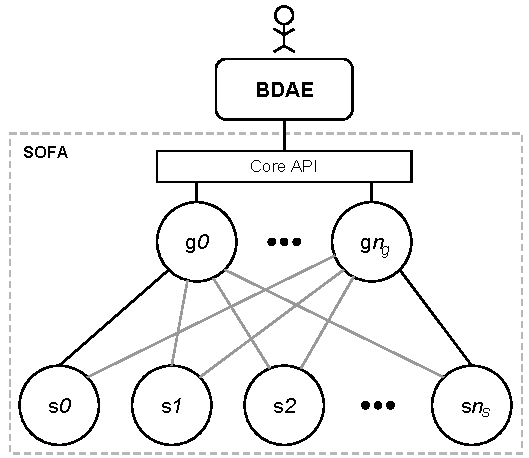
\includegraphics[scale=0.9]{pdf/bdae-overview.pdf}
	\caption[General overview of the BDAE]{General overview of the BDAE integration into \CodeName with same notation as in Figure \ref{fig:sofa-overview}. \label{fig:bdae-overview}}
\end{figure}	


\subsection{Dataset}
The \texttt{SofaBaseObject} (Section \ref{sec:sofabaseobject}) has been extended and delimited along with the requirement of the functions defined in the \texttt{OperationContex}, as a consequence of the chosen execution model. 
\begin{itemize}
	\item A \texttt{MapReduceDataset} has been defined which requires functions executed on the data to be ordered into two categories: \texttt{map} and \texttt{reduce}. 
	\item All functions defined in an extended \texttt{OperationContex} is at runtime verified towards the two categories since the MapReduce execution model prescribes that each operation has at least one map function and at most one reduce function at the end.
\end{itemize}

\section{Collection} \label{sec:collection}
A dataset in \CodeName is defined by a dictionary with metadata and a list of associated semantic blocks, but this metadata structure can with small modifications also be used as a descriptor for a collection of similar datasets, which was one of the objectives (Section \ref{sec:bdae-objectives}):

\begin{quotation}
	\textit{"Define and design a collection structure to batch similar datasets."}
\end{quotation}

In other words; a collection in BDAE is defined as a marginally altered metadata dictionary with zero-length list of associated semantic blocks, that nevertheless obeys the interface of the \texttt{SofaBaseObject}, which is a required for any type of data in \CodeName.

\section{MapReduce}
The tree barrier based operation execution model implemented in \CodeName is well-suited for a MapReduce framework and BDAE is utilizing this straightforward advantage. Figure \ref{fig:reduction-tree} illustrates an example of an execution reduction tree as it would resemble with 16 storage nodes, the figure exemplifies among other things how and when the different storage nodes are communicating to calculate the correct result jointly.
\newline

The joints have an important function in the MapReduce framework and have the overall responsibility of why the execution model adds up and it is implemented as following:
\begin{enumerate}
	\item Each node is executing one or more \texttt{map} functions locally.
	\item The neighbor nodes are based on equation \ref{eq:reduction} calculating the locally combined \texttt{reduce} together.
\end{enumerate}

Figure \ref{fig:map-reduce-tree} illustrates the two steps explained above, where second step is repeated with the same \texttt{reduce} function until all local results are combined to a global result.

\begin{figure}
	\centering
	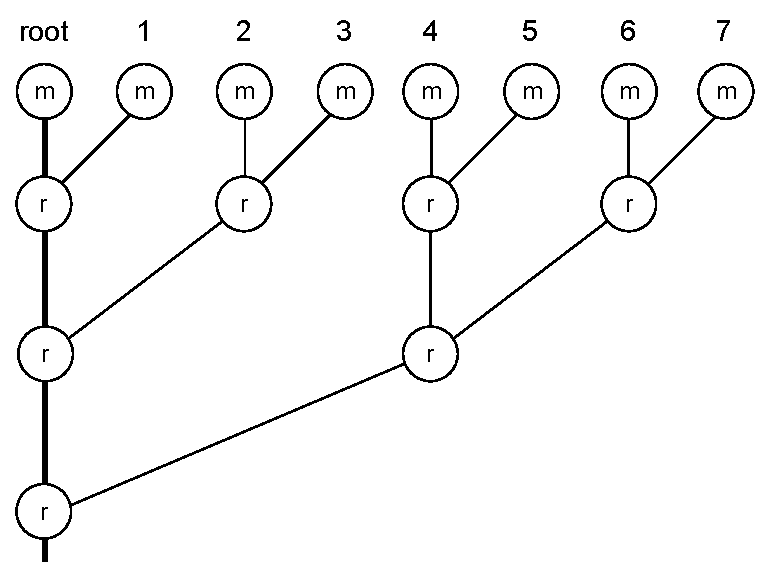
\includegraphics[scale=0.7]{pdf/map-reduce-tree.pdf}
	\caption[BDAE MapReduce implementation]{Utilization of the tree barrier based operation execution model in \CodeName for MapReduce in BDAE. \texttt{m} = map and \texttt{r} = reduce. \label{fig:map-reduce-tree}}
\end{figure}	

\section{User tiers} \label{sec:user-tiers}
One of the objectives for BDAE was to: \textit{"Characterize a domain specific access model"} to first and foremost redeem expectations of system-wide access control, such that the scientist research employees who submit new map reduce operations does not have direct access to boot and teardown servers, as an example.
\newline

The entire BDAE + \CodeName system are divided into three major responsibilities, which each has its domain specific user access level. The responsibilities are inherited as the level increases, which means that the \textbf{data manager} have the same rights as the \textbf{data scientist} and so fourth.
\newline

The core API of \CodeName has been wrapped into a BDAE specific controller that grants access based on user level, in order to restrict the API access and thus accomplish this.

\subsection{Level 1: Data scientist}
Access rights:
\begin{itemize}
	\item Submit new MapReduce operation
	\item Poll for result
	\item Various \texttt{get}-functions to retrieve metadata information regarding the datasets.
\end{itemize}

\subsection{Level 2: Data manager}
Access rights:
\begin{itemize}
	\item Create dataset
	\item Create collection (essentially a thin wrapper around the create dataset API-call with some extra collection specific logic.)
	\item Append data to dataset
	\item Update/delete dataset
\end{itemize}

\subsection{Level 3: System administrator}
Access rights:
\begin{itemize}
	\item Boot and teardown servers
\end{itemize}

\section{Templates} \label{sec:templates}
BDAE provides a range of different abstract templates related to commonly used data types within the field of interest, to reduce excessive workload for the end-users and generalize the final implementation solution, such that solutions to similar problems are easily comparable.
\newline

\noindent
The templates provided includes:
\begin{itemize}
	\item One for \textbf{text} data that can split raw data into semantic blocks by three different properties: \textit{line}, \textit{sentence} or \textit{word}.
	\item A template for \textbf{image} data that simplifies the burden of transforming raw data such as tiff-files into Numpy arrays.
	\item The template for \textbf{Numpy/Bohrium array}'s is a simple solution that uses the template module binder described subsequently to bind regularly used functions from the respective libraries.
	\item One of the objectives listed in Section \ref{sec:bdae-objectives} includes: \textit{"Load complex data structures such as NetCDF $\ldots$ in an intelligent and thus efficiently way to reduce I/O cost."}, which is accomplished by utilizing the collection module (Section \ref{sec:collection}) to create a \textbf{NetCDF} template. This is possible since this data format essentially is a group of related data records. 
\end{itemize}

\subsection{Module binder}
The module binder is not as such a template, but provides opportunities for conveniently binding Python built-in and other third party library functions like \texttt{map} and \texttt{reduce} specific \texttt{OperationContext} functions.
\newline

An example: \texttt{count(}x, y\texttt{)} is a built-in function from the \texttt{string} module in Python \cite{PagePython} that counts number of \texttt{y} in \texttt{x}. The following snippet transforms the \texttt{count(}x, y\texttt{)} into \texttt{count\_occurrences(}x, y\texttt{)} with identical logic parameters and results.
\vspace*{2mm}
\begin{lstlisting}[language=Python, basicstyle=\footnotesize, numbers=none, showtabs=false, showstringspaces=false, showspaces=false, otherkeywords={string,new_fun_names}, stringstyle=\color{blue}]
   module_binder(string, function_binder, ['count'], 
                 new_fun_names=['count_occurrences'])
\end{lstlisting}
\vspace*{-6mm}

\section{Libraries} \label{sec:libraries}
BDAE provides three python libraries one for each of the user tiers (Section \ref{sec:user-tiers}): \texttt{libbdaescientist}, \texttt{libbdaemanager} and \texttt{libbdaeadmin} respectively, that implements the logic listed.

\section{Extensions}
Using the rather simple \CodeName core API it is possible to write useful and comprehensive extensions, as BDAE exemplifies. Likewise it is possible to create extensions on top BDAE using the libraries briefly explained in the previous section. The generic web interface and Android\cite{PageAndroid} application described in this section are two examples of that.

\subsection{Web}
\begin{figure}[h!]
	\centering
	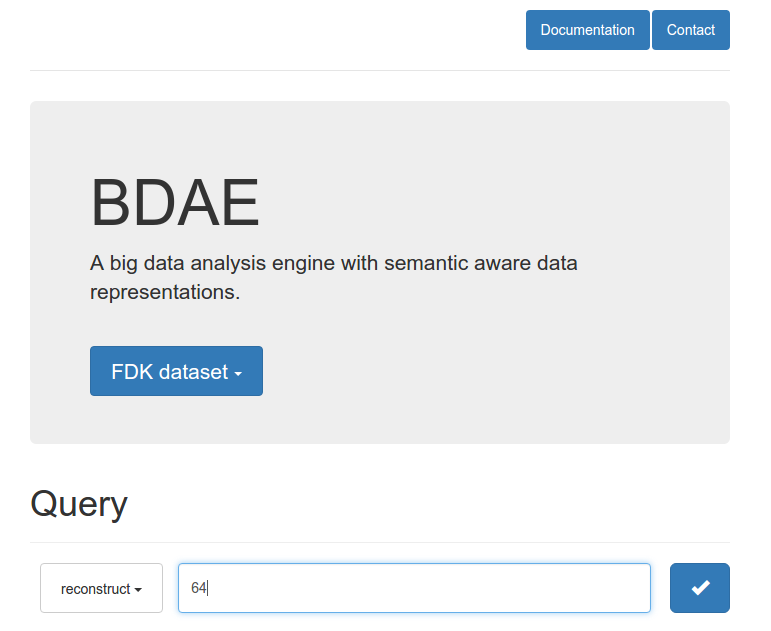
\includegraphics[scale=0.33]{img/website.png}
	\caption{Overview of the BDAE website. \label{fig:website}}
\end{figure}

A simple graphical user interface represented as a website (illustrated in Figure \ref{fig:website}) is provided as part of the BDAE framework installation (explained in Appendix \ref{app:installation}). 
\clearpage

The website expands the options regarding the scientist position, since it is no longer a requirement to master the skill of programming in order to operate BDAE at that user tier. At the moment it is possible to:
\begin{itemize}
	\item Choose the dataset to operate on among all available in \CodeName.
	\item Submit a new MapReduce operation.
	\item And view the result whenever it has finished the execution.
\end{itemize}
, but supporting more features are in the project pipeline.

\subsection{Android application} \label{sec:bdaeapp}
The Android application provides a handheld modern access to the scientist level of BDAE, implemented in a minimalist Google approved material design \cite{PageMaterialDesign} (Figure \ref{fig:app-overview}) (Appendix \ref{chp:app-screenshots}).
\newline

\begin{figure}[h!]
	\centering
	\vspace*{4mm}
	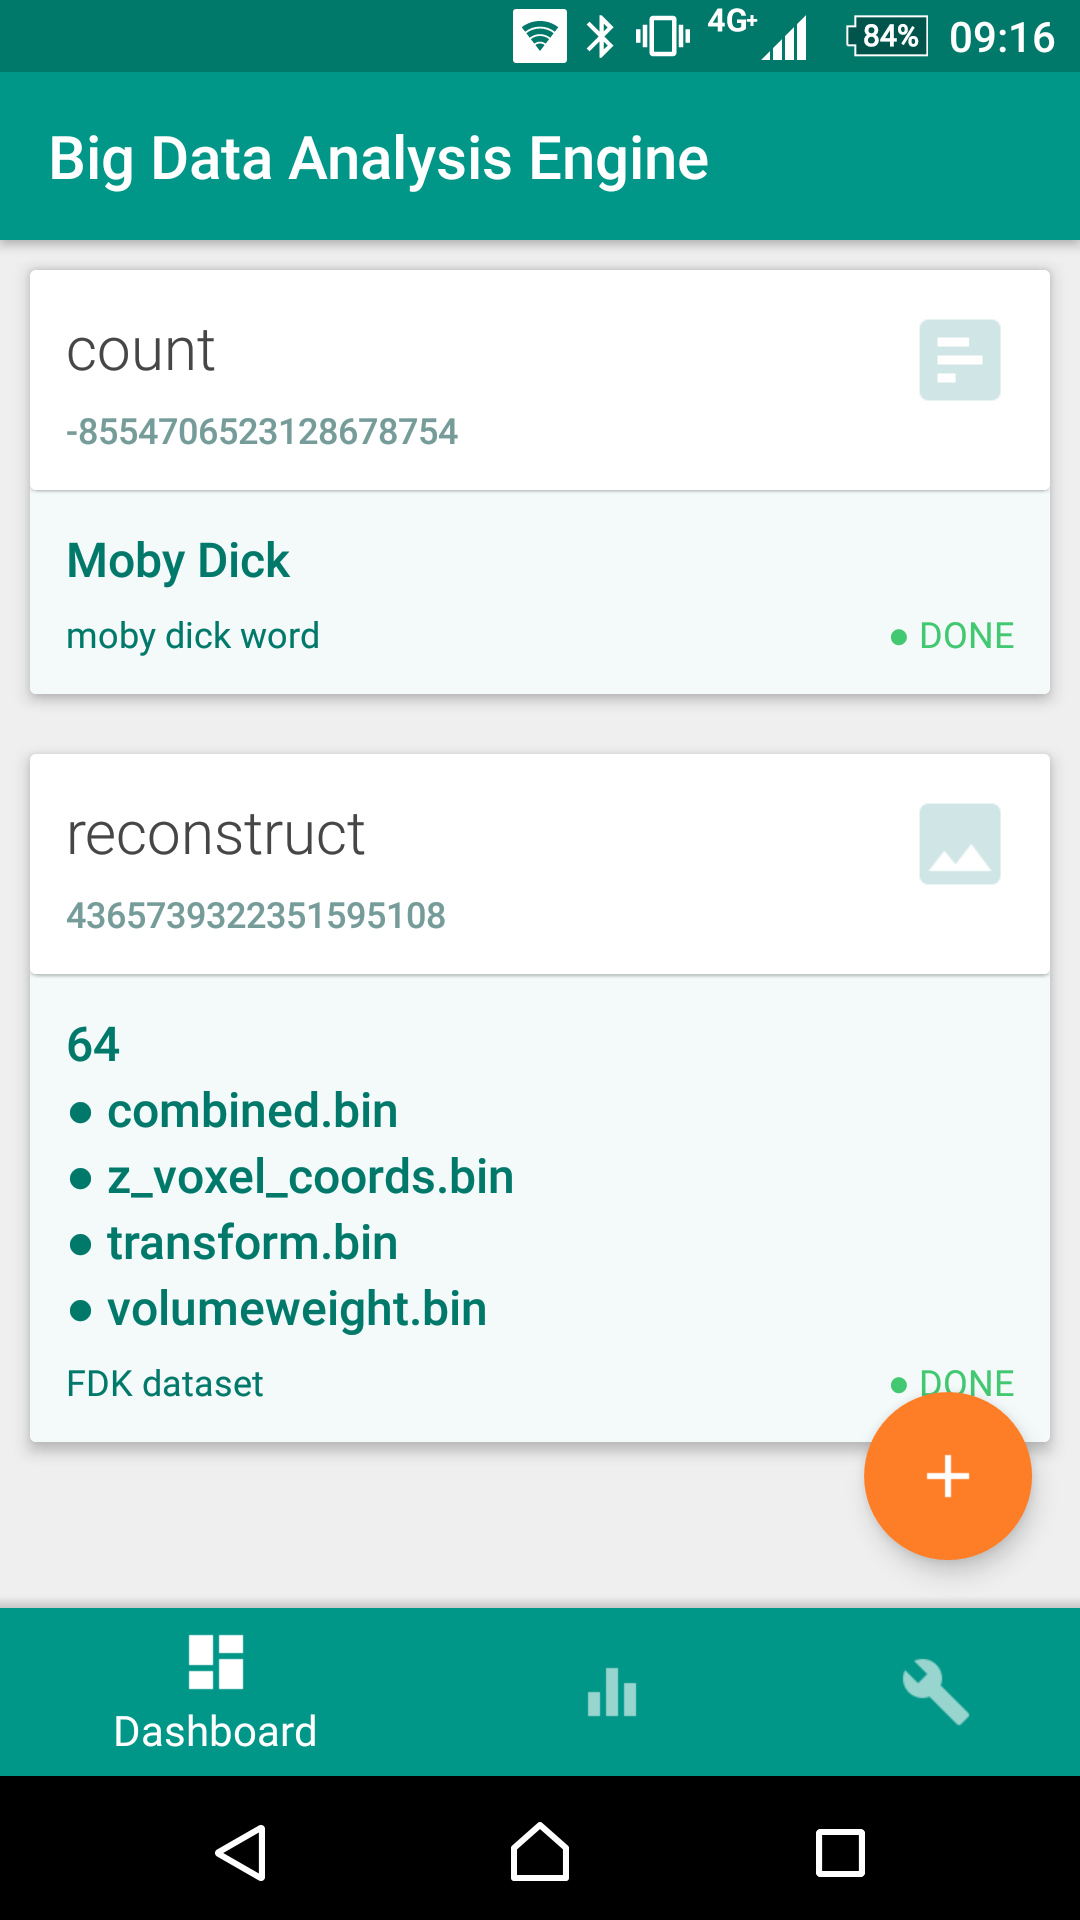
\includegraphics[width=0.4\textwidth]{img/overview.png}
	\caption[Android application overview]{Android application overview of the current MapReduce operations executing in BDAE. \label{fig:app-overview}}
	\vspace*{4mm}
\end{figure}

\noindent
The application supports following features:
\begin{itemize}
	\item Configuration of gateway access server.
	\item All types \CodeName specific instances defined by the \texttt{instance-name} system configuration.
	\item Visualization of current executing MapReduce operations.
	\item Adding new operations for existing datasets.
	\item Listing metadata information about all datasets currently available in \CodeName.
	\item View the results of all the previous executed operations.
\end{itemize}

\section{Blackbox}
One of the useful and productive features in BDAE the ability to transform sequential code into a MapReduce operation with minimal programming effort and without profound knowledge of how the code works. 

All it takes is: 
\begin{itemize}
	\item Identify the reduction part in the original code.
	\item Determine the need for ghosts (Section \ref{sec:operation}).
	\item Describe the data using on the of available BDAE templates (Section \ref{sec:templates}) or by extending the \texttt{MapReduceDataset} (Section \ref{sec:bdae-overview}).
	\item Combine the specified \texttt{map} and \texttt{reduce} functions in a operation (Section \ref{sec:operation}) to produce the expected result.
\end{itemize}

\section{Example}
The productivity, readability and maintainability levels of \CodeName and BDAE are demonstrated and compared to Hadoop since the implemented prototype is a more or less complete framework. Hadoop was chosen based on the popularity and thus comprehensive usage and thereby plenty of very well-produced examples.
\newline

The example used to illustrate the mentioned features of \CodeName and BDAE is a simple processes of log files to summarize the events by type\cite{PageTomWheeler}. This: \texttt{2013-06-29 22:17:05.362 CDT ERROR "Out of memory"} is an example of a log output and thereby a job input for the \texttt{MapReduce} operation. 
\newline

The map and reduce functions are mainly\footnote{Other languages such as Python are available through the Hadoop Streaming API.} written in Java and thus forces an object-oriented class structure of the function logic. The \texttt{Mapper} and \texttt{Reducer} class representations requires specific and hard coded object types of the input and output parameters, partially due to the programming language restrictions but also because that Hadoop sorts the output of the map function before applying the reduce function.

\subsection{Map}
The map function in BDAE implementing the logic described is defined by a simple 5 line code snippet (Code \ref{lst:bdae-map}), whereas the corresponding Hadoop code is specified by 39 lines of code (Appendix \ref{sec:hadoop-map}).

\begin{lstlisting}[float, basicstyle=\fontsize{8}{5}\selectfont\ttfamily, language=Python, xleftmargin=.8cm, caption={BDAE map function}, label={lst:bdae-map}]
def log_mapper(blocks, levels):
    res = zeros((1, len(levels)))
    for entry in sum(blocks, []):
        res += array([entry.count(level) for level in levels])
    return res
\end{lstlisting}

\subsection{Reduce}
The BDAE reduce function is a simple function with 2 lines of code (Code \ref{lst:bdae-reduce}) that calculates the aggregated amount of log events. The corresponding Hadoop code is 25 lines of code (Appendix \ref{sec:hadoop-reduce}).
\vspace*{4mm}

\begin{lstlisting}[basicstyle=\fontsize{8}{5}\selectfont\ttfamily, language=Python, xleftmargin=0.8cm, caption={BDAE reduce function}, label={lst:bdae-reduce}]
def log_reducer(blocks):
    return array(blocks).sum(axis=0)
\end{lstlisting}